\documentclass{beamer}

\mode<presentation> {
\usetheme{Madrid}
}

\usepackage{graphicx}
\usepackage{booktabs} % Allows the use of \toprule, \midrule and \bottomrule in tables
\usepackage[utf8]{inputenc} % Required for inputting international characters
\usepackage[spanish]{babel}
\usepackage[T1]{fontenc} % Output font encoding for international characters
\usepackage{tikz}

%----------------------------------------------------------------------------------------
%	TITLE PAGE
%----------------------------------------------------------------------------------------

\title[Funciones hash]{Funciones Hash e Integridad de datos}

\author{Aarón Arias Pérez}
\institute[UCA]
{
Universidad de Cádiz \\
\medskip
}
\date{\today} % Date, can be changed to a custom date

\graphicspath {{images/}}
\begin{document}

\begin{frame}
\titlepage % Print the title page as the first slide
\end{frame}

%----------------------------------------------------------------------------------------
%	PRESENTATION SLIDES
%----------------------------------------------------------------------------------------


\begin{frame}
\frametitle{Funciones Hash}
\begin{enumerate}
\item ¿Qué son las funciones hash?
\item ¿Para qué se utilizan?
\end{enumerate}

\begin{figure}
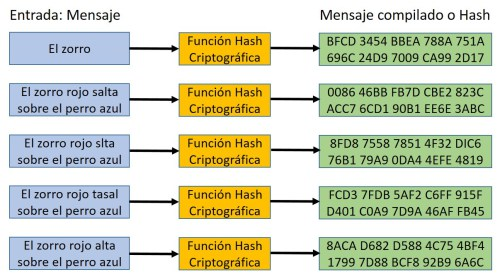
\includegraphics[width=0.8\linewidth]{images/imagen_intro.jpg}
\end{figure}

\end{frame}

%------------------------------------------------

\begin{frame}
\frametitle{Clasificación}

\begin{figure}
\begin{tikzpicture}[sibling distance=10em,
  every node/.style = {shape=rectangle, rounded corners,
    draw, align=center,
    top color=white, bottom color=green!20}]]
  \node {Hash functions}
  	child { node {unkeyed}
			child { node {MDCs}
				child { node {OWHF} }
				child { node {CRHF} }}
			child { node {other applications}}}
    child { node {keyed}
      child { node {other applications}}
      child { node {MACs} } };
\end{tikzpicture}
\caption{Esquema de la clasificación de funciones hash.}
\end{figure}

\end{frame}

%------------------------------------------------

\begin{frame}
\frametitle{Propiedades}
\begin{enumerate}
\item {\LARGE Resistencia a la preimagen}
\item {\LARGE Resistencia a la 2ª preimagen}
\item {\LARGE Resistencia a la colisión}
\end{enumerate}
\end{frame}

%------------------------------------------------

\begin{frame}
\frametitle{Proceso iterativo}
\begin{figure}
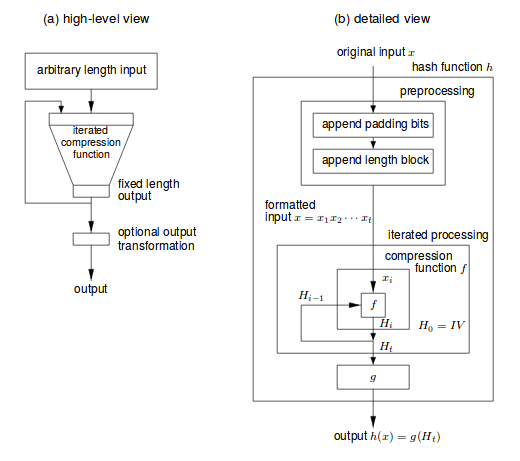
\includegraphics[width=0.8\linewidth]{images/imagen_hashfunction.png}
\caption{Proceso iterativo de la función hash.}
\end{figure}
\end{frame}

%------------------------------------------------

\begin{frame}
\frametitle{Integridad de datos}
\begin{block}{Definición}
  La integridad de datos es la propiedad por la cual los datos no
  han sido alterados de manera no autorizada desde el momento en el que
  fueron creados, transmitidos o almacenados por una fuente autorizada.
\end{block}
\end{frame}

%------------------------------------------------

\begin{frame}
\frametitle{Operaciones que invalidan la integridad}
\begin{itemize}
\item Inserción de bits (incluyendo las que provienen de fuentes fraudulentas)
\item Eliminación de bits
\item Reordenamiento de bits o grupos de bits
\item Inversión o sustitución de bits
\item Cualquier combinación de las anteriores
\end{itemize}
\end{frame}

%------------------------------------------------

\begin{frame}
\frametitle{Importancia del Hashing}
\begin{itemize}
\item Comunicaciones (protección contra intrusos y integridad de datos)
\item Bases de datos (contra accesos indeseados)
\item Estructuras de datos mas eficientes en búsqueda (tablas resumen, árboles Merkle)
\end{itemize}
\end{frame}

%------------------------------------------------

\begin{frame}
\frametitle{Referencias}
\footnotesize{
\begin{thebibliography}{99} % Beamer does not support BibTeX so references must be inserted manually as below
\bibitem[HAC, 1996]{p1} Alfred J. Menezes, Paul C. van Oorschot and Scott A. Vanstone (1996)
\newblock Handbook of Applied Cryptography
\end{thebibliography}
}
\end{frame}

%----------------------------------------------------------------------------------------

\end{document}
